\section{Optimised Implementation}
In order to optimise the na\"ive implementation the execution time for each line was investigated using line_profiler. The result of running the line_profiler on the na\"ive implementation can be seen in \autoref{AppLinePS1}. As can be seen in \autoref{AppLinePS1} the line that takes the absolute longest to execute per hit are the lines which calls the function that creates the histograms. Therefore, this was the first thing to be improved. This was done by utilising the Numpy function for generating histograms. Once this was done the script was much faster as can be seen in \autoref{AppLinePS2}. However, when inspecting the histograms after this alteration it seemed an issue had been introduced. The histogram showed that certain bins were eliminated, as can be seen in \autoref{fig:HistEli}. 

\begin{figure}[h]
\centering
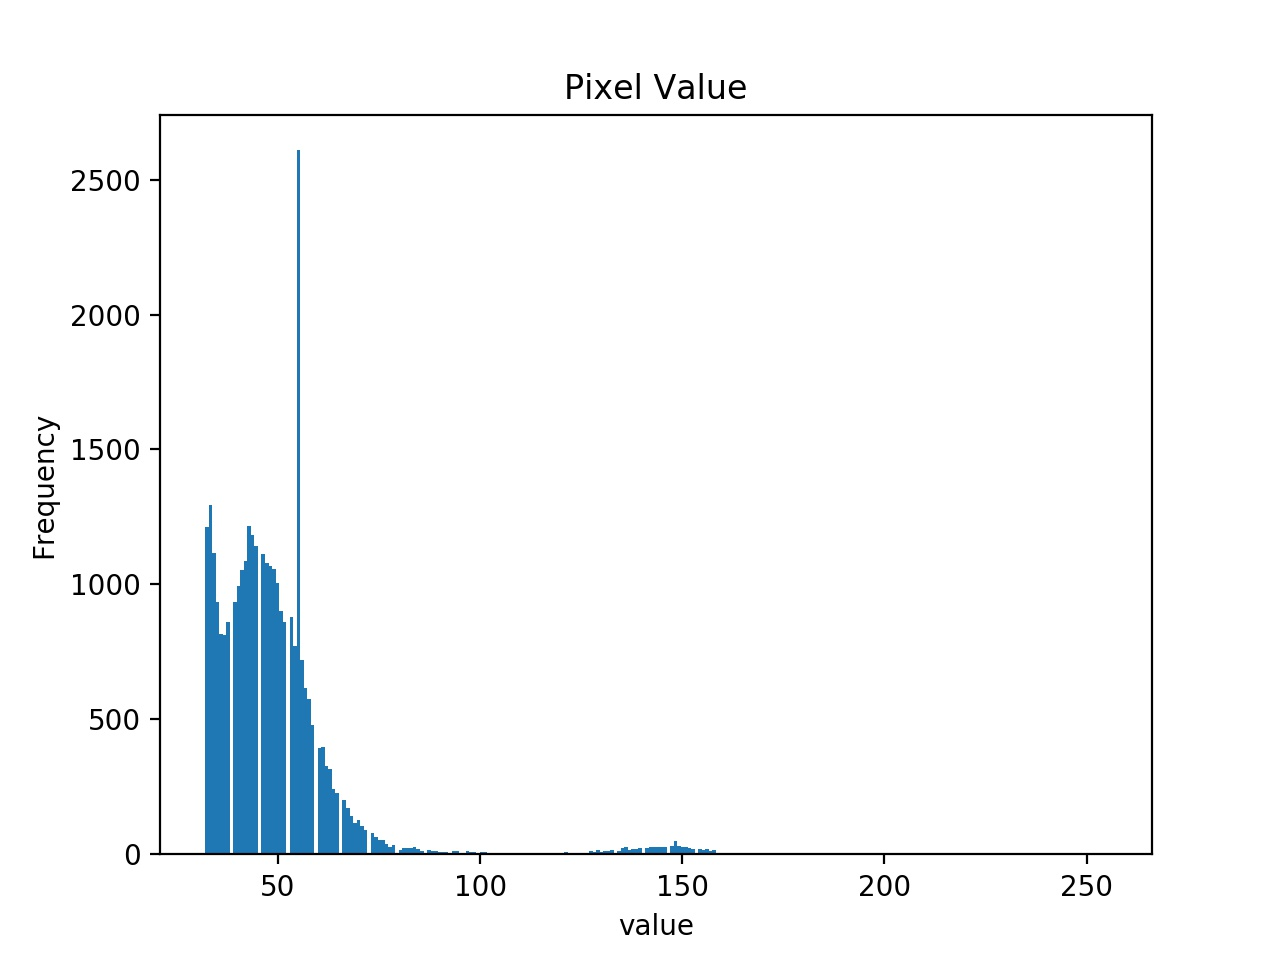
\includegraphics[width=\textwidth]{figures/hist_troublespacing.jpg}
\caption{The histogram of the reconstructed image with eliminated values.}
\label{fig:HistEli}
\end{figure}

\noindent
Eventually it turned out that this was due to the fact that the numpy.histogram adapts the range of the histogram to the range of the present values if no range is specified. This was easily solved by passing a range as an argument to the histogram function. The range in this case had to be specified as range(0,256). 
Another thing that took quite some time with the total amount of hits was finding the thresholded pixels and their coordinates using a for loop. This was optimised using a simple logical operation and the numpy.where function. This made it somewhat faster. In the noise remover function there are also quite a lot of if statements taking some time to execute. One hit does not take a lot of time, but the if statements are called a lot and therefore it takes a lot of time in total. Therefore this would be nice to optimise, however, to the extend of the available knowledge optimisation was not possible. \\

In the equalise histogram function the lines taking the longest time in total, besides the histogram, were the lines setting the pixels higher or lower than $ 255 $ or $ 0 $ to those values. Therefore some effort was put into optimising those lines. The lines were gradually optimised to a better and less time consuming solution. The process can be tracked in \autoref{AppLinePS22} and \autoref{AppLinePS24} and the final source code of the optimised implementation is found in \autoref{AppOpt}.